\documentclass[tikz,border=10pt]{standalone}
% Scale: s = 0.0181 cm per px, centred on ink bbox centre (245,170)
\begin{document}
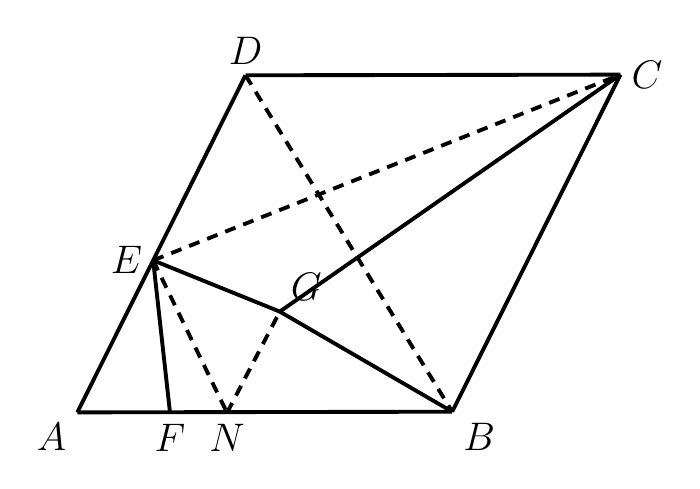
\begin{tikzpicture}[line width=1.4pt, line join=round, font=\fontsize{14.5}{17.4}\selectfont]
  % Named points (converted from pixel coordinates)
  \coordinate (A) at (-3.476458792520792,-2.13077207907025);
  \coordinate (B) at (1.2849317602850732,-2.1224659491558753);
  \coordinate (C) at (3.4210682397149146,2.1584659491558815);
  \coordinate (D) at (-1.34032231309095,2.150159819241507);
  \coordinate (E) at (-2.513218894388246,-0.20038774017126376);
  \coordinate (F) at (-2.299,-2.136);
  \coordinate (G) at (-0.905,-0.851);
  \coordinate (N) at (-1.575,-2.136);

  % Outer parallelogram edges
  \draw (A) -- (E) -- (D);
  \draw (D) -- (C);
  \draw (C) -- (B);
  \draw (B) -- (A);

  % Solid inner edges
  \draw (E) -- (F);
  \draw (E) -- (G) -- (B);
  \draw (C) -- (G);

  % Dashed edges
  \draw[dash pattern=on 4pt off 3pt] (E) -- (C);
  \draw[dash pattern=on 4pt off 3pt] (D) -- (B);
  \draw[dash pattern=on 4pt off 3pt] (E) -- (N);
  \draw[dash pattern=on 4pt off 3pt] (N) -- (G);

  % Labels
  \node[above right] at (G) {$G$};
  \node[below] at (N) {$N$};
  \node[below] at (F) {$F$};
  \node[left] at (E) {$E$};
  \node[below left] at (A) {$A$};
  \node[above] at (D) {$D$};
  \node[right] at (C) {$C$};
  \node[below right] at (B) {$B$};
\end{tikzpicture}
\end{document}